%%%%%%%%%%%%%%%%%%%%%%%%%%%%%%%%%%%%%%%%%%%%%%%%%%%%%%%%%%%%%%%%%%%%%%%
%%%%%%%%%%%%%%%%%%%%%%%%%%%%%%%%%%%%%%%%%%%%%%%%%%%%%%%%%%%%%%%%%%%%%%%
%%%%%                                                                 %
%%%%%     <file_name>.tex                                             %
%%%%%                                                                 %
%%%%% Author:      <author>                                           %
%%%%% Created:     <date>                                             %
%%%%% Description: <description>                                      %
%%%%%                                                                 %
%%%%%%%%%%%%%%%%%%%%%%%%%%%%%%%%%%%%%%%%%%%%%%%%%%%%%%%%%%%%%%%%%%%%%%%
%%%%%%%%%%%%%%%%%%%%%%%%%%%%%%%%%%%%%%%%%%%%%%%%%%%%%%%%%%%%%%%%%%%%%%%


\chapter{Experimental Results}

\section{Performance Evaluation}

\subsection{Logging and SD-card driver} \label{logging_perf}

Experimental evaluation of the SD-card driver by visualising write operations using an oscilloscope attached to the SPI bus revealed an important trade-off that greatly impacts the performance of the logging driver. Although many overheads are introduced by the FAT file system, the SD card also introduces an overhead during read and write operations. As write operations are more relevant in this particular application the following will examine only write operations.

Figure~\ref{fig:sd_card_write} illustrates the initial steps of writing to an SD-card. First a write command is issued. This is then followed by one or more data packets consisting of a data token, 1-2048 bytes of data and two CRC bytes. Between the cursors in Figure~\ref{fig:sd_card_write} one data packet is transmitted. Once all the data packets have been transmitted, a write termination command is transmitted. This last command is omitted if a single block write operation is used.

\begin{figure}[H]
    \centering \includegraphics[width=1.0\textwidth]{./figures/"SPI SD WRITE".PNG}
    \caption{Write command and data packet on SPI bus with SD card.}
    \label{fig:sd_card_write}
\end{figure}

Between each data packet and after the full sequence of packets and commands, the SD card enters a busy state where it is processing the written data. As Figure~\ref{fig:sd_card_write_wait} shows, the busy time after the full sequence (or rather after the write termination command) is particularly long in relation to the transmission time of a single data packet.

\begin{figure}[H]
    \centering \includegraphics[width=1.0\textwidth]{./figures/"SPI SD WRITE1".PNG}
    \caption{Wait time after writing data packet to SD card.}
    \label{fig:sd_card_write_wait}
\end{figure}

Further testing revealed that, while the busy time between data packets is very small, the total busy time is almost completely dominated by the busy time at the end of a write operation. This is further verified by another test where chunks of different sizes are repeatedly written to a file in the FAT file system and the data rate observed. Table~\ref{tab:write_speed} shows the results of this test. As can be seen from Figure~\ref{fig:write_speed} the write speed behaves almost linearly compared to the chunk size.

\begin{table}[htbp]
    \caption{Write speeds for chunks of different sizes.}
    \label{tab:write_speed}
    \centering\begin{tabular}{@{}lcr@{}} \toprule
    \textbf{Chunk size} & \textbf{Average data-rate} \\ \midrule
        256 bytes & 21 kB/s \\
        512 bytes & 41 kB/s \\
        1024 bytes & 80 kB/s \\
        2048 bytes & 148 kB/s \\
        4096 bytes & 254 kB/s \\ \bottomrule
    \end{tabular}
\end{table}

\begin{figure}[H]
\centering
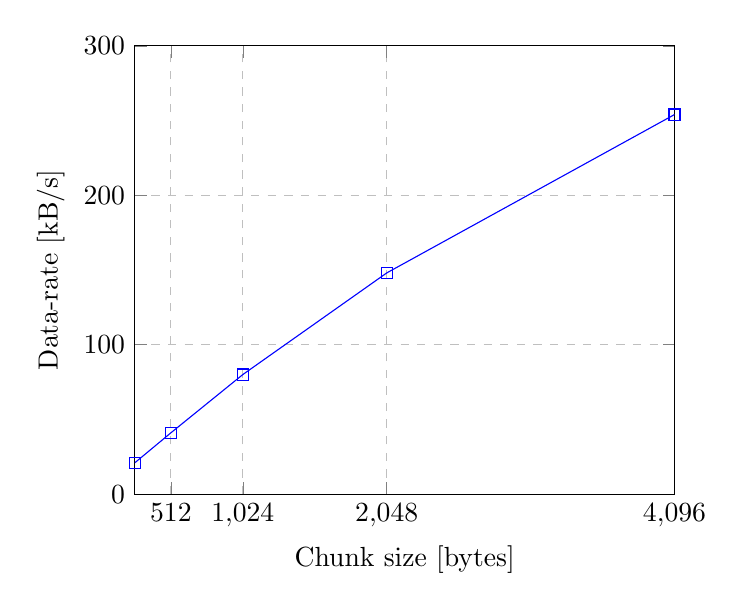
\begin{tikzpicture}
\begin{axis}[
    xlabel={Chunk size [bytes]},
    ylabel={Data-rate [kB/s]},
    xmin=256, xmax=4096,
    ymin=0, ymax=300,
    xtick={512,1024,2048,4096},
    xmajorgrids=true,
    ymajorgrids=true,
    grid style=dashed,
]
 
\addplot[
    color=blue,
    mark=square,
    ]
    coordinates {
    (256,21)(512,41)(1024,80)(2048,148)(4096,254)
    };
 
\end{axis}
\end{tikzpicture}
\caption{Write speeds for chunks of different sizes.}
\label{fig:write_speed}
\end{figure}

Given these results we have a memory/data-rate trade-off. Memory is limited on the micro-controller but we also want to maximise the amount of data that can be logged. In-field experimentation showed that under most circumstances write buffers of 2048 bytes are sufficient to achieve the data-rate necessary to log all sensor data. Nonetheless, we ended up using buffers of 4096 bytes to insure that no data would be lost.

\subsubsection{Comparison to Escher}

The most important objective in comparison to Escher was to improve the logging system. Already by introducing event-based logging more infrequent measurements can be logged less than more frequent measurements. As a result, higher data rates for more important data can be achieved by reducing the bandwidth used by less important measurements. More dramatically, the redesigned system logged on average 1355 data points per second at a data-rate of 29 kB/s, while the system on Escher achieved only a constant rate of 173,5 data points per second.

\begin{figure}[H]
\centering
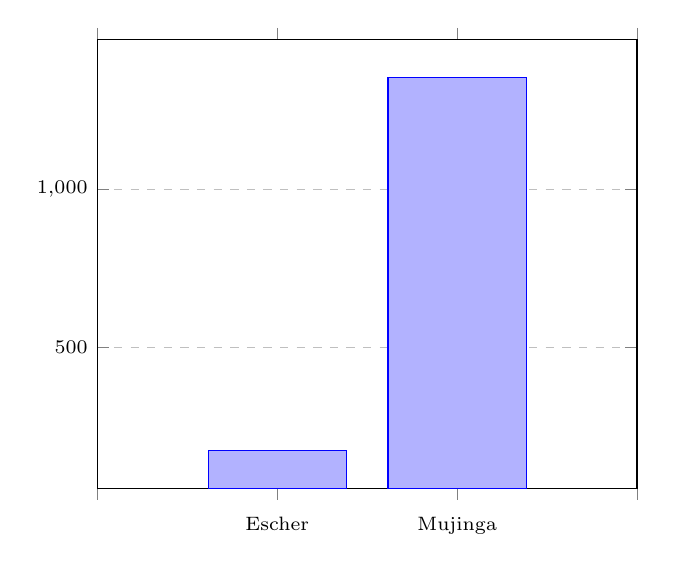
\begin{tikzpicture}
\begin{axis}[
        ybar,
        xtick={0,1,2,3},
        xticklabels={,Escher,Mujinga,},
        xticklabel style={yshift=-0.1cm},
        tick label style={font=\scriptsize},
        xmin=0,
        xmax=3,
        ymajorgrids=true,
        grid style=dashed,
        bar width=50pt
    ]

\addplot [
        blue,fill=blue!30
    ]
    coordinates {
        (1,173.5)(2,1355)
    };
\end{axis}
\end{tikzpicture}
\caption{Average number of logged data points per second.}
\label{fig:write_speed}
\end{figure}

\subsection{Networking}

Using an oscilloscope the SPI bus with the micro-controller and Ethernet controller can be monitored. Figures ~\ref{fig:net_send} and ~\ref{fig:net_recv} visualise the sequence of commands necessary for sending and receiving short 12 byte network packets. In order to send a packet, the micro-controller must first read the write pointer it should use from the Ethernet controller. Then it can write to the Ethernet controller's packet RAM at the write address. It must then update the write pointer so the Ethernet controller knows the length of the packet and finally confirm the packet using a send command. The sequence for receiving packets is analogous. Notice however, that the process is triggered by the interrupt signal from the Ethernet controller.

\begin{figure}[H]
    \centering \includegraphics[width=1.0\textwidth]{./figures/"SPI NET SEND".PNG}
    \caption{Command sequence for sending a network packet on SPI bus.}
    \label{fig:net_send}
\end{figure}

From Figure~\ref{fig:net_send} we can see that it takes only 39 microseconds to complete all commands necessary to send a network packet of this size at maximum clock rate supported by the SPI interface (12,5 MHz). The use of the DMA controller leads to uninterrupted transmission of each command on the bus. Although the demonstrated performance is more than fast enough for this application, the driver could still be optimised to reduce the time between commands. Some of the computation necessary for the next command is performed after the previous command is transmitted. Although this would increase memory usage, it could be performed while the previous command is still transmitting. On the other hand, for longer packets the time is dominated by the transmission subsequence labelled "write packet" in Figure~\ref{fig:net_send}.

The same optimisation could be applied to the reception of network packets but again Figure~\ref{fig:net_recv} shows that the full sequence only takes 47 microseconds, which is sufficient for this application. 

\begin{figure}[H]
    \centering \includegraphics[width=1.0\textwidth]{./figures/"SPI NET RECV".PNG}
    \caption{Command sequence for receiving a network packet on SPI bus.}
    \label{fig:net_recv}
\end{figure}

\section{In-Field Evaluation and Competition}

The control system was implemented specifically for the Hyperloop Pod Student Competition. It was extensively tested before the competition during functional tests and on a test 150m test track in Switzerland. During the competition the software was tested in several tests, most notably the functional test, navigation test and state diagram test.

\subsection{Pre-competition testing}

After checking the correct operation of all sensors and actuators in conjunction with the software, we checked that all emergency conditions and safety features worked correctly. Next, full pod operation was tested in a vacuum chamber. We were successfully able to spin up the motors in vacuum and all components operated nominally during the test. The pressurized battery compartments remained pressurized and the cells were therefore not damaged.

In addition to the vacuum chamber test, the team was able to use a 150m test track designed to match the specifications of the test tube at the competition. We completed several runs demonstrating correct operation of the navigational sensors, the navigation algorithm, the control of the inverters using both speed and torque commands, the control of the brake system and telemetry transmission and logging. Further test runs focused on applying maximal acceleration over short distances in order to fine-tune traction control.

\subsection{Competition}

\begin{figure}[H]
  \centering 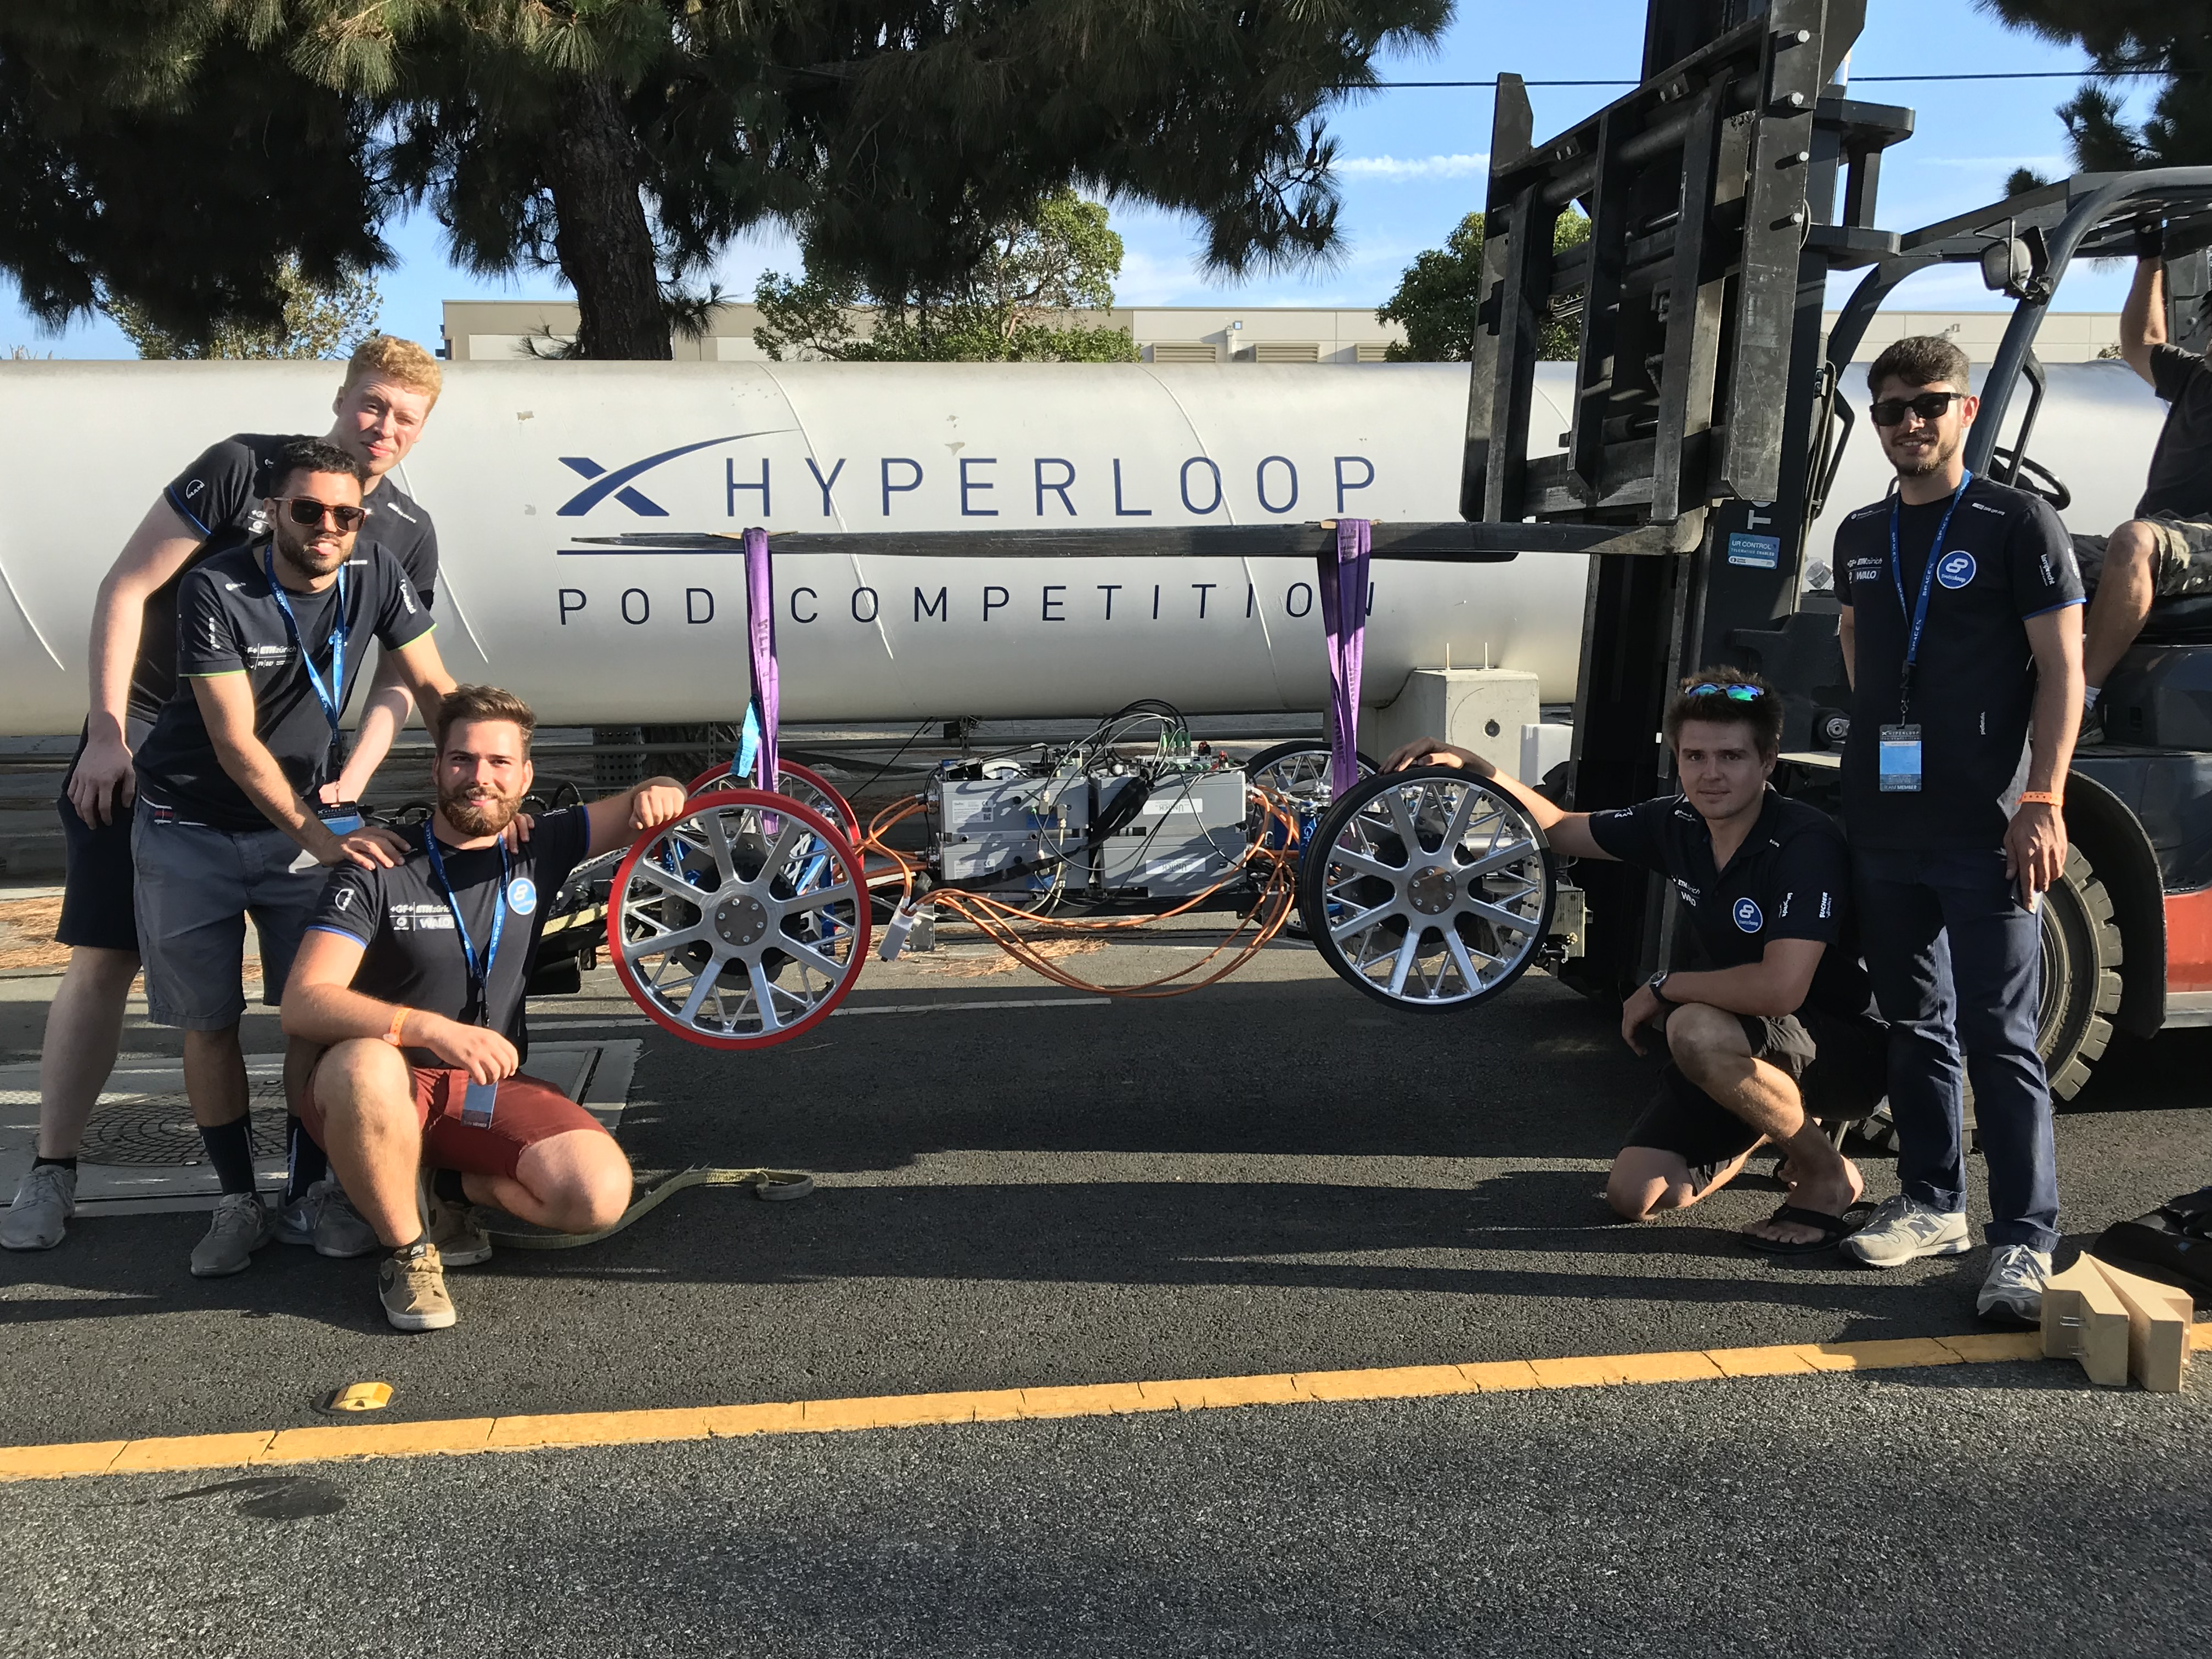
\includegraphics[width=1.0\textwidth]{./figures/mujinga_competition}
  \caption{Picture of Mujinga without shell in front of the Hyperloop test tube in Los Angeles.}
\end{figure}

Throughout the competition week the pod was subjected to a wide range of tests. Three tests specifically target the control software developed in this thesis.

First, the functional test ensures that after power-on the pod is in a safe state and telemetry is received with nominal values. During this test the team also demonstrated correct operation of all safety-critical pod functions such as the brakes from software and using the control panel to command the pod.

Next, the navigation test verifies that the navigational mechanisms built into the software work correctly and the level of fault tolerance is assessed. In order to show correct functionality of the navigational algorithm, all possible scenarios were simulated using fake optical markings while the pod remained stationary and the software responses were observed using the telemetry data visualised in the control panel.

Finally, the state diagram test consists of verifying the pod operates according to the state diagram (Figure~\ref{fig:state_diagram}). Essentially, this test checks that the global finite state machine is correctly implemented. To demonstrate this, all automatic transitions are tested by simulating all possible causes for the transition. For example, the transition \texttt{RUN} $\rightarrow$ \texttt{BRAKING} should occur after the pod has travelled a pre-defined distance. This can be simulated by passing fake optical markings in front of the laser contrast sensors.

\begin{figure}[H]
  \centering 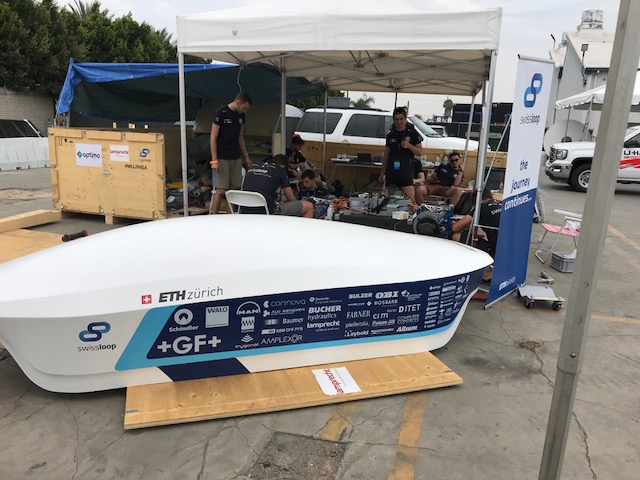
\includegraphics[width=1.0\textwidth]{./figures/mujinga_competition_tent}
  \caption{Picture of Mujinga's shell in front of the tent where the team worked on the pod during testing week at SpaceX.}
\end{figure}

With all these tests passed, the team had actually gained a decent lead compared to the other teams in the competition. The next test for the pod was the vacuum chamber test, where the full pod is placed in a large vacuum chamber. Although this test had been previously carried out successfully in Switzerland, the pod suffered a sever failure during this test preventing the team from advancing to the finals of the competition.

Shortly after enabling the high-voltage systems in vacuum, a loss of communications occurred. After re-pressurising the vacuum chamber it was immediately possible to see that the low-voltage electronics had been fatally damaged. Further investigation revealed, that the high-voltage batteries had been short circuited. Surprisingly, the low-voltage systems continued to log data for a full second after the failure. After analysing the data, the failure could be narrowed down to one of the inverters. A manufacturing fault caused arcing to occur between the two battery poles. The arcing damaged the inverter, portions of the low-voltage electronics, the low-voltage battery and both high-voltage batteries. Although we were able to repair all other components, the high-voltage battery cells were too severely damaged from the over-current to be safely used any further.

\section{Conclusion}

%Objective

The objective of this bachelor thesis was to design a control system for a prototype Hyperloop pod competing in SpaceX's 2018 Hyperloop Pod Competition. The safety and therefore the correctness and reliability of the system was the highest priority. The system had to be robust and be able to execute many runs of the pod without needing intervention. The implementation also had to improve on the software of the previous pod Escher, in particular by simplifying the system, reducing bottlenecks, being able to log significantly more data and being designed from the ground up with testability in mind.

%Platform

The platform chosen for this project was based on a Texas Instruments Launchpad together with a custom interface PCB. The software makes use of both CPUs of the dual-core micro-controller and the built-in Control Law Accelerator for parallel processing. No real-time operating system was used. Instead, the system is designed to be fundamentally asynchronous. Modular software design and a centralized data-flow make it easily maintainable and extendible.

%Networking

To provide remote telemetry data and control, a protocol was designed that is resistant to unstable network connections and packet loss. An external Ethernet Controller allows the computational effort of running a full network stack to be offloaded from the CPU. Communication with the Ethernet Controller runs over an SPI bus and the driver makes use of DMA to provide near optimal performance. The networking driver is a dual-core implementation and uses IPC flags to synchronise communication between CPU cores. Experimental evaluation showed that the performance far surpassed the requirements of the project.

%Logging

In order to log data to an SD card, several file systems were considered. In order to simplify retrieving log data as much as possible, the FAT file system was chosen. To this end, an SD-Card driver was implemented using the FIFO extension of the SPI interface. Event-based logging allows for variable and mixed data-rates. Similar to the networking driver, logging is a dual-core process using IPC flags for synchronisation. Experimental evaluation revealed a memory/data-rate trade-off where more memory usage can lead to increased data-rates. On average though, the logging system was able to log 7,8 times more data than the logging system on Escher. In order to visualise large amounts of log data rapidly and efficiently, a custom plotting application was developed.

%External ADC
%RS485 Bus
%CAN Bus

Although most sensors were chosen with digital outputs, some produce analog output signals. These are read using an external analog to digital converter for particularly accurate readings. The driver for the external ADC is highly optimized and operates with optimal communication. Communication with the laser distance sensors runs over two RS485 buses, which allow several sensors to share a single bus. The drivers use the FIFO extension of the micro-controller's serial interface for efficient and asynchronous operation. A sequence of interrupts allows the RTS signal to be controlled asynchronously. Some remaining devices communicate using a CAN bus. The micro-controller's built-in CAN interface and a driver library from Texas Instruments again allowed for an efficient and asynchronous implementation.

%Control

A robust navigation algorithm was implemented with failure recovery and filtering to allow reliable, safe and autonomous control of the pod. A global finite state machine was designed and implemented to control all safety critical processes and incorporates all checks necessary to guarantee safety of the vehicle. The states and state transitions are optimised for testability, by reducing the number of automatic transitions to a minimum.

%Competiton

In conclusion, the control system developed in this thesis was able to meet all design objectives. Performance was evaluated experimentally and surpassed the requirements of the project. The system was successfully deployed and used to control Mujinga before and during the 2018 Hyperloop Pod Competition hosted by SpaceX in Los Angeles. Although the team was not able to advance to the finals due to a manufacturing fault, the system performed perfectly during tests and therefore can be considered a success.

\section{Outlook}

The control software was designed to be modular and easily extendible, so it will serve as a basis for future systems as Swissloop continues to develop Hyperloop technology, striving for efficient high-speed transport. While Mujinga does not yet represent a viable pod for a full-scale commercial Hyperloop system, it tackles some of the challenges relating to high-speed transport in a low-pressure environment. Ongoing work at Swissloop will allow for future iterations that will become increasingly close to a full-scale solution.
